One thing I have tried to do in class is show the students how
generative AI has been developing at a phenomenal rate. This is an
example of something spat out by \href{https://www.bing.com/create}{Bing
Image Creator} of a much higher quality than before:

\begin{figure}
\centering
\pandocbounded{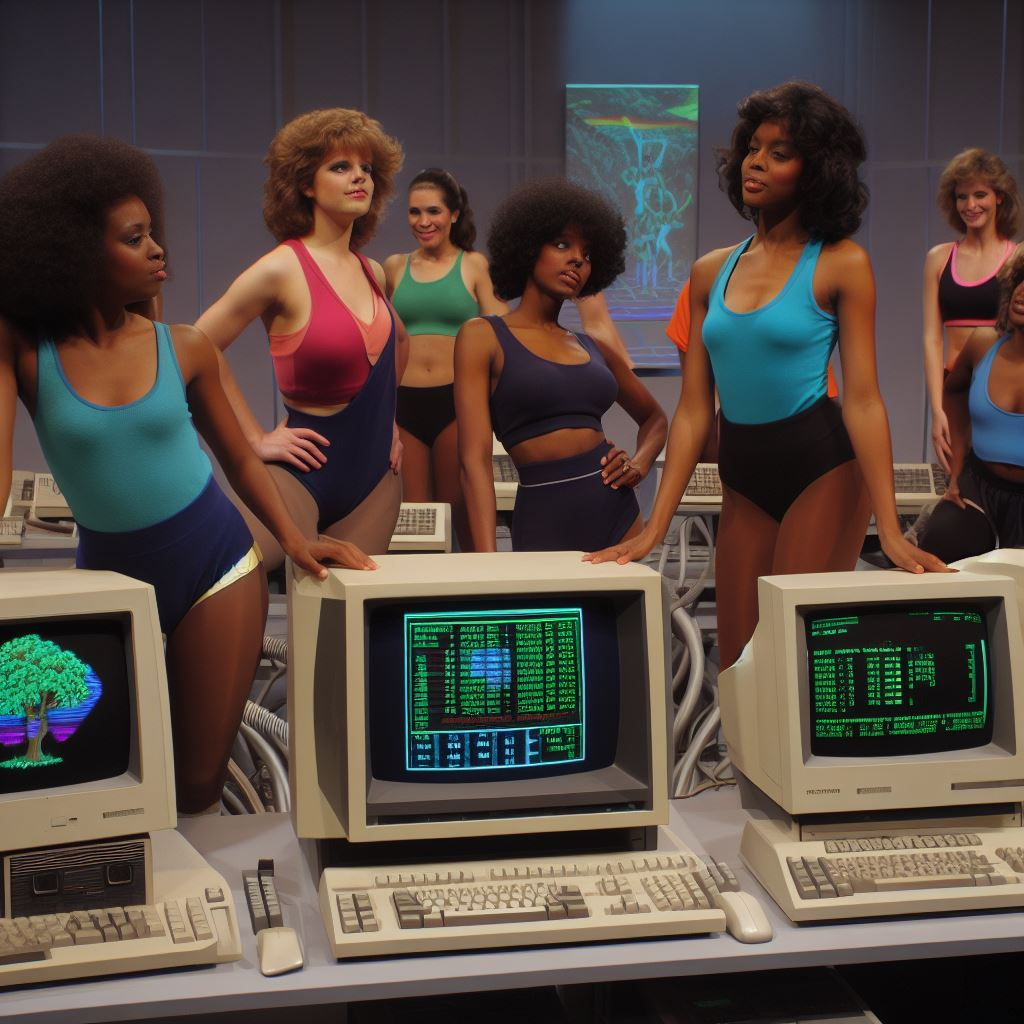
\includegraphics[keepaspectratio]{\%7B\%7Bsite.url\%7D\%7D/img/quantified.jpg}}
\caption{Image generated by the following prompt given to Bing Image
Creator: ``A lost scene from the iconic public television program''The
Computer Chronicles'' where the hosts show us a variety of 1980s
computer technologies for the first time that help promote physical
fitness. They are joined by multiple female physical fitness
enthusiasts.''}
\end{figure}

\begin{quote}
\emph{Image generated by the following prompt given to Bing Image
Creator: ``A lost scene from the iconic public television program''The
Computer Chronicles'' where the hosts show us a variety of 1980s
computer technologies for the first time that help promote physical
fitness. They are joined by multiple female physical fitness
enthusiasts.''}
\end{quote}

Stewart and Gary seem to be missing from the picture, though. The system
generates premium nightmare fuel, too. For example:

\begin{figure}
\centering
\pandocbounded{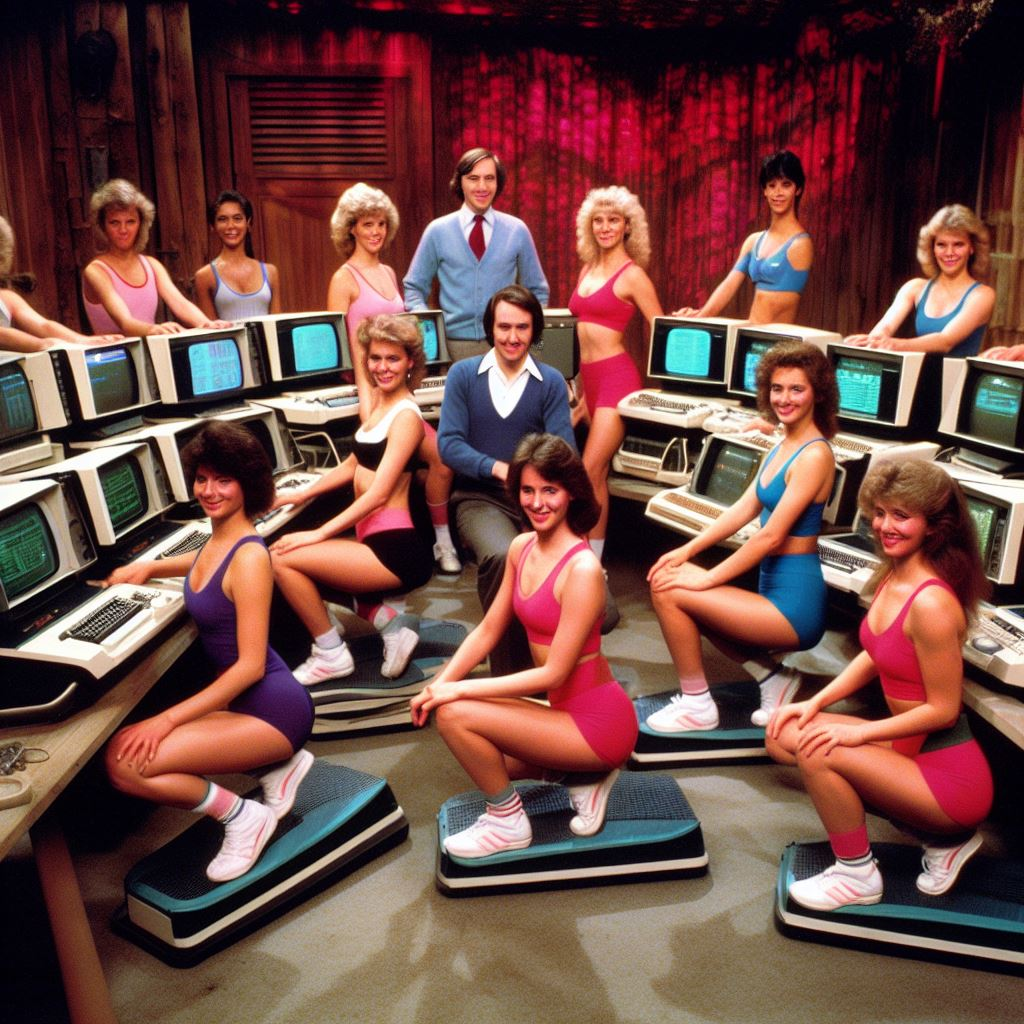
\includegraphics[keepaspectratio]{\%7B\%7Bsite.url\%7D\%7D/img/nightmarez.jpg}}
\caption{Image generated by the following prompt given to Bing Image
Creator: ``A lost scene from the iconic public television program''The
Computer Chronicles'' where the hosts show us a variety of 1980s
computer technologies for the first time that help promote physical
fitness. They are joined by multiple female physical fitness
enthusiasts.''}
\end{figure}

You might've seen this sort of picture in a computer magazine from the
late 1980s or early 1990s touting the benefits of ``the quantified
self'', I suppose.

Things are starting to get really, really world in the generative AI
space, I think.
